\emph{Iceberg, DOI: X, DATE}

\section{THE SURFACE OF AN AQUAPLANET
GCM}\label{the-surface-of-an-aquaplanet-gcm}

Martin jucker

ARC Centre of Excellence for Climate Extremes and Climate Change
Research Centre, University of New South Wales, Sydney, Australia

Reviewed by

\section{Abstract}\label{abstract}

This article describes some of the challenges and culprits of working
with a mixed layer ocean and trying to arrive at an acceptable
climatology with a minimum number of parameters.\\
We discuss why even the simplest version of the Model of an idealized
Moist Atmosphere \href{https://github.com/mjucker/MiMA}{MiMA}
\href{http://journals.ametsoc.org/doi/10.1175/JCLI-D-17-0127.1}{Jucker
and Gerber (2017)} includes meridional heat flux (``Q-flux''), a
meridionally inhomogeneous mixed layer depth, options to reduce the
mixed layer depth locally (``land''), as well as options to change
surface albedo.

This work is licensed under a
\href{http://creativecommons.org/licenses/by/4.0/}{Creative Commons
Attribution 4.0 International License}.

\subparagraph{Keywords}\label{keywords}

climate science, general circulation models, mixed layer ocean, slab
ocean

\section{Introduction}\label{introduction}

Studying the effects of the stratosphere and its coupling to the
troposphere in idealised general circulation models (GCMs) has
traditionally been restricted to dry models, where the temperature is
simply forced to a prescribed relaxation temperature profile (e.g.
\href{http://journals.ametsoc.org/doi/abs/10.1175/1520-0477(1994)075\%3C1825:APFTIO\%3E2.0.CO;2}{Held
and Suarez (1994)},
\href{http://www.agu.org/pubs/crossref/2002/2001GL014284.shtml}{Polvani
and Kushner (2002)},
\href{http://journals.ametsoc.org/doi/abs/10.1175/JAS-D-12-0305.1}{Jucker
\emph{et al.} (2013)}). Although idealised moist models have existed for
some time in the form of gray radiation models (e.g.
\href{http://journals.ametsoc.org/doi/abs/10.1175/JAS3753.1}{Frierson
\emph{et al.} (2006)}, or
\href{https://doi.org/10.1175/2007JCLI2065.1}{O'Gorman and Schneider
(2008)}), the stratosphere adds some complexity in terms of vertical and
meridional structures which are non-trivial to add to such models.

There was an obvious gap to close in the model hierarchy between the
gray radation schemes and full GCMs, which required the inclusion of the
radiative effects of stratospheric ozone. Therefore, Ed Gerber and I
decided to build the Model of an idealized Moist Atmosphere (MiMA),
which represents one step up from the Frierson gray radation model
{[}\href{http://journals.ametsoc.org/doi/abs/10.1175/JAS3753.1}{Frierson
\emph{et al.} (2006)},
\href{http://journals.ametsoc.org/doi/abs/10.1175/JAS3935.1}{Frierson
\emph{et al.} (2007)}{]} by replacing the gray radiation with the full
radiative transfer code RRTM (Rapid Radiative transfer Model,
\href{http://doi.wiley.com/10.1029/97JD00237}{RRTM, Mlawer \emph{et al.}
(1997)}). A short introductory movie for MiMA can be found in Fig. 1.

\href{http://www.youtube.com/watch?v=8UfaFnGtCrk}{\includegraphics{http://img.youtube.com/vi/8UfaFnGtCrk/0.jpg}}\\
Figure 1: A 30-second introduction to the Model of an idealized Moist
Atmosphere (link to YouTube).

Naively, this means simply starting from Frierson's model and exchanging
the call to radiation. Everything else could be left as is, as the model
has been used very successfully for many studies involving moist
dynamics.

In particular, the existing moist model had a boundary layer scheme
based on Monin-Obukhov similarity theory, a simplified Betts-Miller
convection scheme as well as a mixed layer ocean where shortwave solar
radiation gets absorbed and re-emitted as in the longwave. All of these
simplified parameterisations of real processes have been carefully
built, tuned and tested by the original authors, and it was not our
intent to modify them.

\section{Mixed layer ocean}\label{mixed-layer-ocean}

As might be expected with a model which explicitly solves the full
radiative transfer including the shortwave, the role of the mixed layer
is rather important: Instead of simply acting as lower boundary for the
dynamic atmosphere (plus source of water vapor), it has to properly
absorb incoming shortwave radiation, convert the absorbed energy into
surface temperature, and then re-radiate in the longwave according to
its temperature. As a result, the parameter settings which worked for
the gray radiation scheme might not work in MiMA.\\
Indeed, it soon turned out that by far most of the development time of
MiMA went into the mixed layer rather than the new radiation scheme.

\subsection{The seasonal cycle}\label{the-seasonal-cycle}

\href{http://journals.ametsoc.org/doi/abs/10.1175/JAS3753.1}{Frierson
\emph{et al.} (2006)} use a mixed layer depth of 10m. If MiMA is run
with the same depth, and setting the radiation to Earth's astronomical
parameters (obliquity, solar constant, rotation rate, radius), the poles
will heat a lot during summer and cool a lot during winter (Fig. 2,
solid blue line). In some cases, this can cause the simulation to fail
as the moist dynamics cannot deal with the much too low temperatures
over the winter pole.

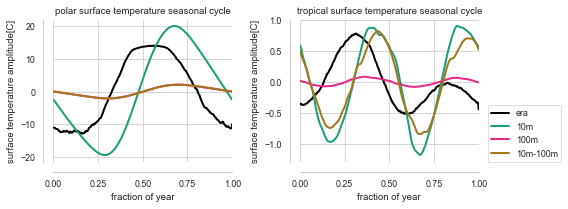
\includegraphics{ts_amp.png}\\
Figure 2: polar (70-90°N) and tropical (15°S-15°N) temperature
timeseries at different mixed layer depths.

Thus, the mixed layer should be increased at least until the poles do
not cause the simulation to fail. For realistic polar temperatures in
both winter and summer it should be increased even more. There is a
trade-off between robustness of the model (i.e.~most parameters can be
changed and the model still runs smoothly) and realism as compared to
e.g.~ERA-Interim reanalysis. Our emphasis is on stability more than
realism, and we found a value of about 100 meters to be about right.
Note that with this setting, the seasonal cycle over the poles has a
much lower amplitude than observed, but this also reduces the effects of
the time lag between the model and observations (compare black solid
line to blue and green solid lines in Fig. 2).

With such a deep mixed layer, the model starts being very stable.
Unfortunately, it causes the tropics to be too stable: The InterTropical
Convergence Zone (ITCZ) does not show any real seasonal cycle anymore
but simply sticks to the equator (Figs. 2 and 3). The little that it
does move is lagged by about three months with respect to the solar
forcing, such that such important things as the tropical monsoons around
the globe are delayed by weeks to months (Fig. 2, dashed lines).

Therefore, depending on which phenomena are important for a given
research project, the mixed layer should either be deep or shallow. The
most realistic cases are obtained if the mixed layer is shallow in the
tropics (10-20m), and deep at the poles (50-100m). Therefore, the heat
capacity of the mixed layer can be adjusted to be constant or to have
different values in the tropics and the poles, with a linear transition
region in-between (Fig. 3).

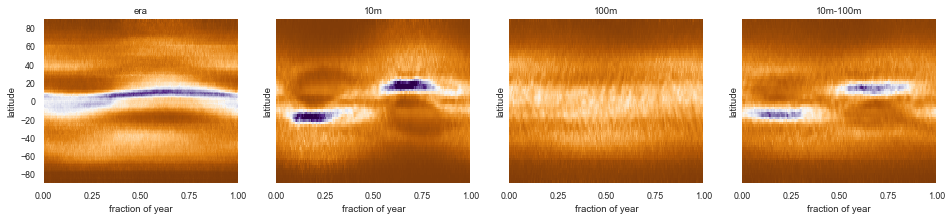
\includegraphics{itcz.png}\\
Figure 3: With a meridionally varying mixed layer depth (right most
panel), the ITCZ can move and follow peak solar input more freely, while
the poles do not become too cold nor too warm.

Here again, there are trade-offs to consider. For instance, shallow
tropics allow a greater movement of the ITCZ over the year, but it also
results in a much broader region of intense precipitation in latitude
(Fig. 3, panel 2). Including a gradient to deeper mixed layer at high
latitudes (panel 4) restricts that meridional extension of the ITCZ.

\subsection{Effect of land}\label{effect-of-land}

MiMA has the option of adding ``land'' in the sense of reduced mixed
layer depth (the heat capacity of rock is about one thousand times lower
than that of water). As a zeroth order approximation, land therefore is
still an infinite source of water vapour to the atmosphere. This can
either be in the form of an external file (containing a a land-sea mask
as is often used in comprehensive models), slaving it to surface
topography (by setting an altitude threshold above which any grid point
is considered land), or by adding arbitrary rectangles or patches of
land (Fig. 4). Then, one can define a different heat capacity for any
grid points considered land. As a consequence, whenever adding land, the
zonal mean heat capacity is lowered, and the effect of this new mixed
layer depth distribution should first be tested before conducting
research with the chosen setup. For instance, using a realistic land
mask will add the Antarctic continent at the South Pole, which,
depending on the setup, might cause problems at high southern latitudes
because the South Pole now suddenly has a very low heat capacity (see
above discussion).

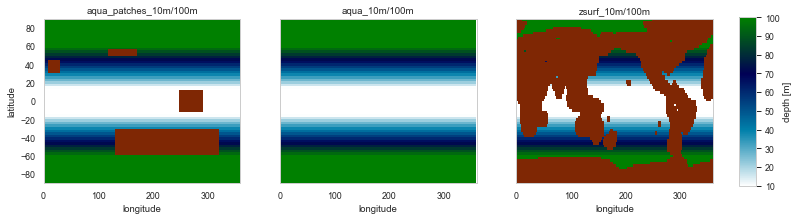
\includegraphics{heat_cap.png}\\
Figure 4: Different land configurations in MiMA. One can add rectangular
``patches'' of land (left), no land at all (middle), or let the land
mask be a function of orography height (right). It is also possible to
provide an input file with a land mask.

\subsection{Ocean heat transport}\label{ocean-heat-transport}

As a consequence of neglecting any ocean dynamics is that the incoming
solar energy is not transported to the poles as efficiently as often
desired (note that the ocean dominates global meridional heat transport
in the tropics \href{https://doi.org/10.1175/2007JCLI1936.1}{Fasullo and
Trenberth (2008)}). As a result, the ITCZ is very narrow and the
tropical-extratropical temperature contrast is rather high. Therefore,
as described by
\href{http://journals.ametsoc.org/doi/abs/10.1175/JCLI-D-11-00716.1}{Merlis
\emph{et al.} (2013)}, a meridional heat flux (``Q-flux'') has to be
introduced manually. In MiMA, this is done with a simple exponential and
zonally symmetric profile following the above paper, and in the cousin
model framework \href{https://execlim.github.com/Isca}{Isca}, either an
external file can be read or a sophisticated algorithm deployed to
adjust the heat flux such that the sea surface temperature (SST) matches
a reference state
\href{https://www.geosci-model-dev.net/11/843/2018/}{Vallis \emph{et
al.} (2018)}.

One thing to keep in mind here is that the simple default Q-flux is
zonally symmetric, and is also active over any regions considered
``land'' as defined above. Thus, if one strives for realism in the
simulated climate and uses real topography and land-sea mask, one might
also think about either not using any Q-flux at all or providing an
input file with more a sophisticated structure. The upcoming version 2.0
of MiMA has seen some development in that direction and includes more
realistic Q-fluxes which are zero over (realistic) land.

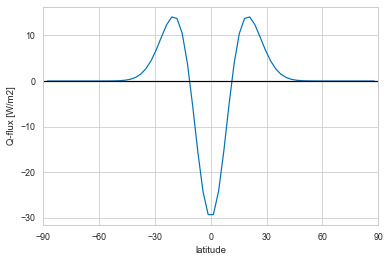
\includegraphics{qflux.png}\\
Figure 5: Default meridional ocean heat transport. Meridional width and
amplitude are runtime input parameters.

\subsection{Albedo}\label{albedo}

Another \emph{a priori} missing component of MiMA is sea ice and snow
cover. This is not a major shortcoming since ocean dynamics,
biogeochemistry and others are willingly left out as well to keep the
model simple. The main effect of ice and snow on atmospheric dynamics is
arguably the albedo effect. Luckily, the albedo can be adjusted rather
easily to account for ice, at least in a static sense. Fig. 6 shows
examples of adding higher albedo south of 65°S to mimic the effect of
Antarctica (yellow line) and different implemented choices for
meridional albedo profiles.

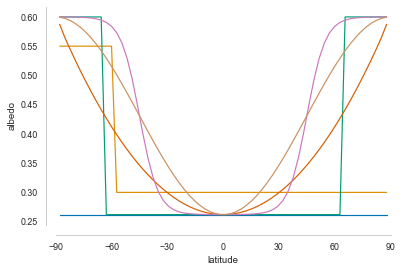
\includegraphics{albedo.png}\\
Figure 6: Illustration of different meridional albedo profiles in MiMA.

\section{Conclusions}\label{conclusions}

The Model of an idealized Moist Atmosphere (MiMA)
{[}\href{http://journals.ametsoc.org/doi/10.1175/JCLI-D-17-0127.1}{Jucker
and Gerber (2017)},
\href{http://mjucker.github.io/MiMA}{mjucker.github.io/MiMA}{]} is a
medium-complexity atmospheric circulation model which was purposefully
built to be as simple as possible while still realistically simulating
the effects of moisture (except clouds) and stratospheric dynamics. The
lower boundary condition is a mixed layer ocean, which is the simplest
surface for such a model. No ocean dynamics is included. During the
development of MiMA, most of the coding, testing, and decision making
was related to the mixed layer ocean, even though it is ``only'' a
boundary condition and does not receive much attention when describing
the model. However, many aspects of the simulated climate depend on the
exact setup of the mixed layer, and most of the knowledge in how to
properly set up this lower boundary is unpublishable personal expertise.
This is true of any atmospheric model set up with a mixed layer ocean as
lower boundary condition. As a result, the author estimates that most
new users are bound to encounter the same difficult decisions and
pitfalls as the users before them.

This paper shows some of the effects of the most important parameters
using MiMA as example: For every new setup, care has to be taken to the
choice of mixed layer depth and its two-dimensional distribution, ocean
heat flux parameterisations, albedo, and the definition and distribution
of land.

Note that the default setup for MiMA (at least version 1) is constant
mixed layer depth. This is to make it as simple as possible, not to make
it as realistic as possible. This will be amended for version 2.0 of
MiMA.

\section{Acknowledgments}\label{acknowledgments}

The author acknowledges the support by the ARC Centre of Excellence for
Climate Extremes under grant CE170100023 and ARC grant FL150100035.\\
ERA-Interim data obtained from
\url{http://apps.ecmwf.int/datasets/data/interim_full_daily/} on
16/07/2015. It was converted to netcdf and made available to the author
by ARCCSS ARC Centre of Excellence for Climate System Science
www.climatescience.org.au.

\emph{Iceberg, DOI: X, DATE}

\begin{center}\rule{0.5\linewidth}{\linethickness}\end{center}

\section{Comments}\label{comments}
